\documentclass{article}

\usepackage{graphicx}
\usepackage{tikz}
\usepackage{tikzsymbols}
\usetikzlibrary{calc,patterns,shapes.geometric}
\pagestyle{empty}
\usepackage[margin=0pt]{geometry}
\geometry{papersize={14in,12in}}

\def\centerarc[#1](#2)(#3:#4:#5){\draw[#1] ($(#2)+({#5*cos(#3)},{#5*sin(#3)})$) arc (#3:#4:#5);}

\begin{document}
	\begin{figure}
		\centering
		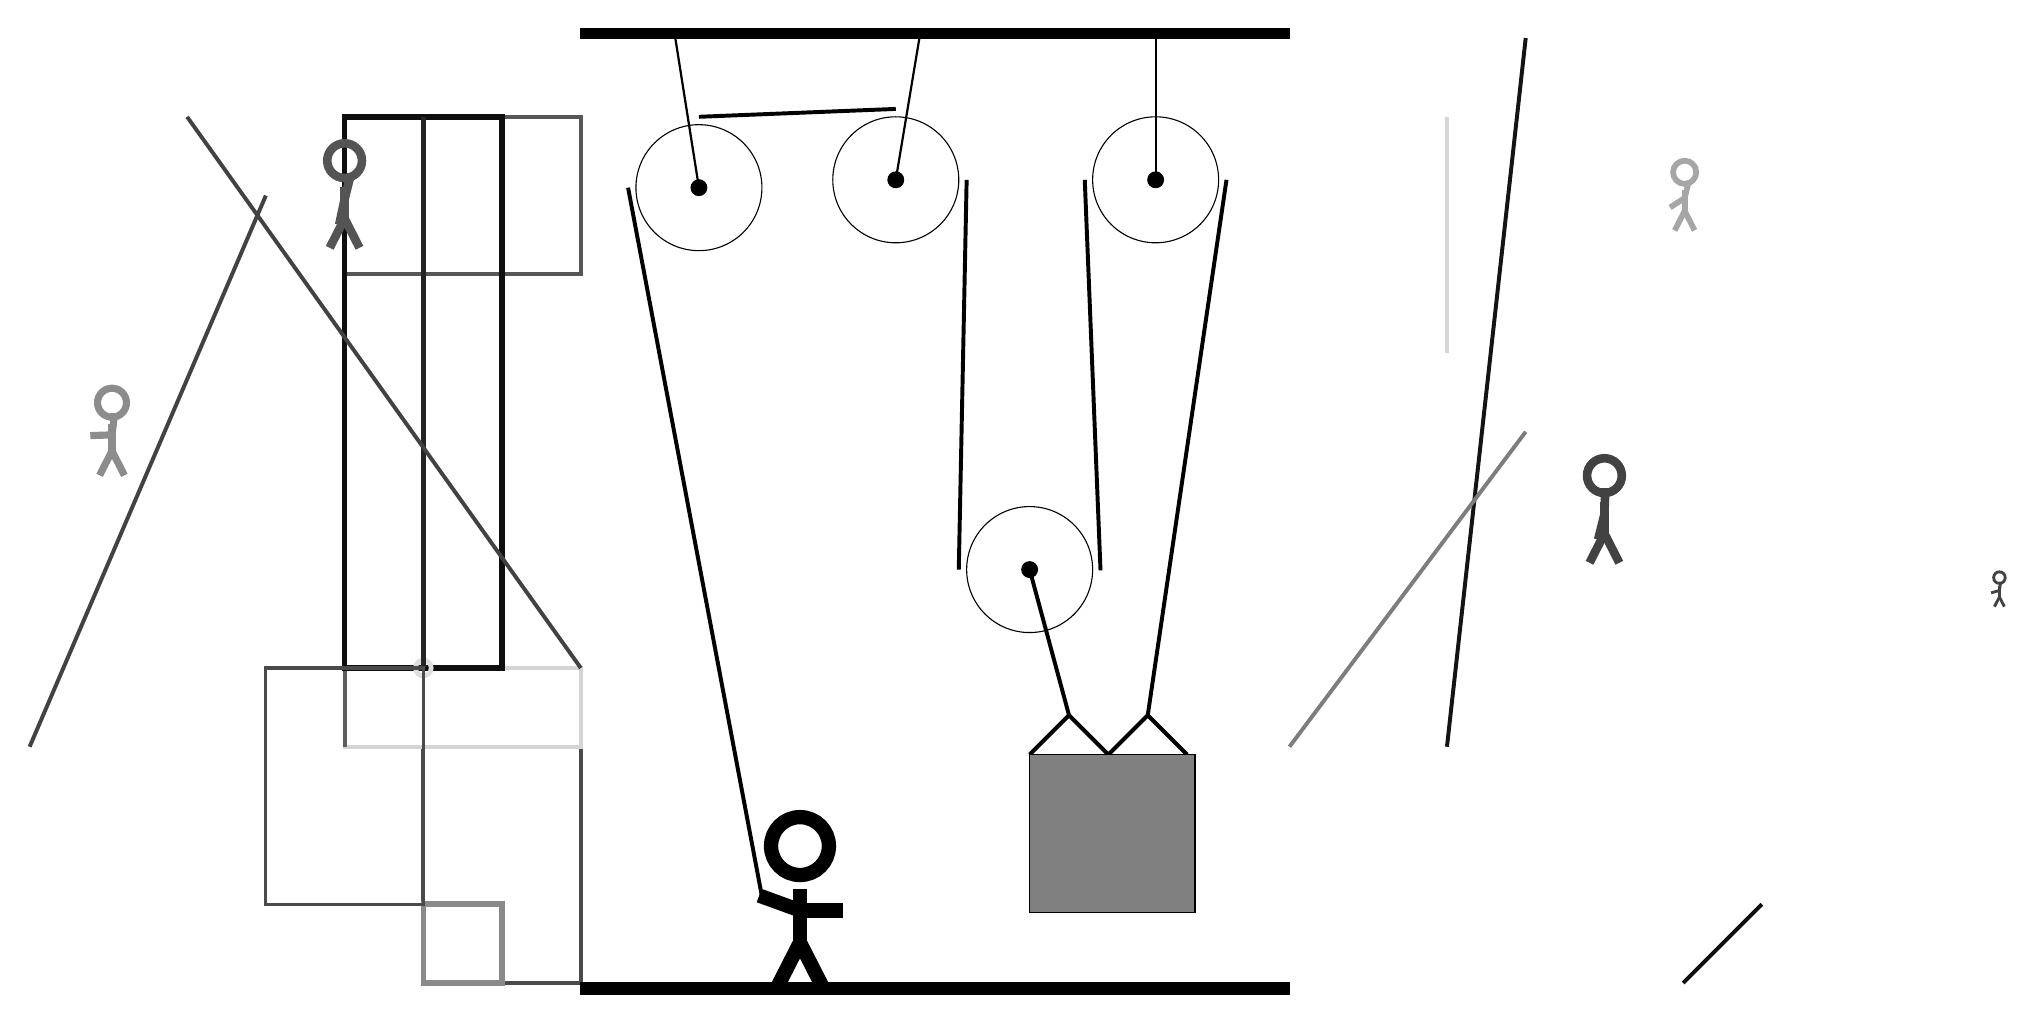
\begin{tikzpicture}
			%%%%% START %%%%%
			
			\draw[fill=black] (-3, 9) rectangle (6, 9.125);
			
			\draw (1, 7.2) circle (0.8);
			\draw[fill=black] (1, 7.2) circle (0.1);
			\draw[thick] (1, 7.2) -- (1.3, 9);
			
			\draw (4.3, 7.2) circle (0.8);
			\draw[fill=black] (4.3, 7.2) circle (0.1);
			\draw[thick] (4.3, 7.2) -- (4.3, 9);
			
			\draw (2.7, 2.25) circle (0.8);
			\draw[fill=black] (2.7, 2.25) circle (0.1);
			
			\draw[line width=0.5mm]  (2.7, -0.1) -- (3.2, 0.4) -- (3.7, -0.1) -- (4.2, 0.4) -- (4.7, -0.1);
			\draw[fill=black!50] (2.7, -0.1) rectangle (4.8, -2.1);
			
			\draw (-1.5, 7.1) circle (0.8);
			\draw[fill=black] (-1.5, 7.1) circle (0.1);
			\draw[thick] (-1.5, 7.1) -- (-1.8, 9);
			
			\draw[line width=0.5mm, color=black!71] (-3, 0) rectangle (-5, -3);
			
			\draw[line width=0.5mm, color=black!74](-7, 7) -- (-10, 0);
			\draw[line width=0.5mm, color=black!92](9, 9) -- (8, 0);
			\node[line width=0.2mm, color=black!45] at (-9, 4) {\Strichmaxerl[5][2][83]};
			\draw[line width=0.5mm, color=black!17] (-3, 1) rectangle (-6, 0);
			
			\draw[line width=0.5mm, color=black!66] (-3, 8) rectangle (-6, 6);
			\draw[line width=0.2mm, color=black!32] (-4, 5) rectangle (-4, 2);
			
			\draw[line width=0.5mm, color=black!63](-6, 0) -- (-6, 5);
			\draw[line width=0.5mm, color=black!51](9, 4) -- (6, 0);
			
			\draw[line width=0.7mm, color=black!94] (-4, 8) rectangle (-6, 1);
			\node[line width=0.5mm, color=black!74] at (10, 3) {\Strichmaxerl[6][76][88]};
			\draw[line width=0.5mm, color=black!94](11, -3) -- (12, -2);
			\node[line width=0.6mm, color=black!74] at (15, 2) {\Strichmaxerl[2][16][82]};
			
			\draw[line width=0.7mm, color=black!46] (-5, -2) rectangle (-4, -3);
			\draw [line width=0.6mm, color=black!13](-5, 1) circle (0.1);
			\draw[line width=0.7mm, color=black!86] (-5, 8) rectangle (-5, 1);
			
			\node[line width=0.3mm, color=black!67] at (-6, 7) {\Strichmaxerl[6][78][76]};
			\draw[line width=0.4mm, color=black!71] (-5, 1) rectangle (-7, -2);
			\node[line width=0.6mm, color=black!35] at (11, 7) {\Strichmaxerl[4][33][76]};
			
			\draw[line width=0.5mm, color=black!74](-3, 1) -- (-8, 8);
			\draw[line width=0.4mm, color=black!16] (8, 5) rectangle (8, 8);
			
			\draw[line width=0.5mm](-0.7, -1.9) --  (-2.4, 7.1);
			\centerarc[line width=0.5mm](-1.5, 7.1)(90:180:0.9);
			\draw[line width=0.5mm](-1.5, 8.0) -- (1, 8.1);
			\centerarc[line width=0.5mm](1, 7.2)(0:90:0.9);
			\draw[line width=0.5mm](1.9, 7.2) -- (1.8, 2.25);
			\centerarc[line width=0.5mm](2.7, 2.25)(180:370:0.9);
			\draw[line width=0.5mm] (3.6, 2.24) -- (3.4, 7.2);
			\centerarc[line width=0.5mm](4.3, 7.2)(0:180:0.9);
			\draw[line width=0.5mm](4.2, 0.4) -- (5.2, 7.2);
			\draw[line width=0.5mm] (3.2, 0.4) -- (2.7, 2.25);
			
			\node at (-0.2, -2) {\Strichmaxerl[10][-20][0]};
			
			\draw[fill=black] (-3, -3) rectangle (6, -3.15);
			
			%%%%% END %%%%%
		\end{tikzpicture}
	\end{figure}	
\end{document}